\documentclass{article}[10pt]
\usepackage{multicol, enumerate, enumitem, hyperref, color, soul, setspace, parskip, fancyhdr, amssymb, amsthm, amsmath, bbm, latexsym, units, mathtools}
\everymath{\displaystyle}
\usepackage[headsep=0.5cm,headheight=0cm, left=1 in,right= 1 in,top= 1 in,bottom= 1 in]{geometry}

\begin{document}
This is the Answer Key for Module 6 Version C.

26. Which of the following equations \textit{could} be of the graph presented below?
$$  $$ 
\begin{center}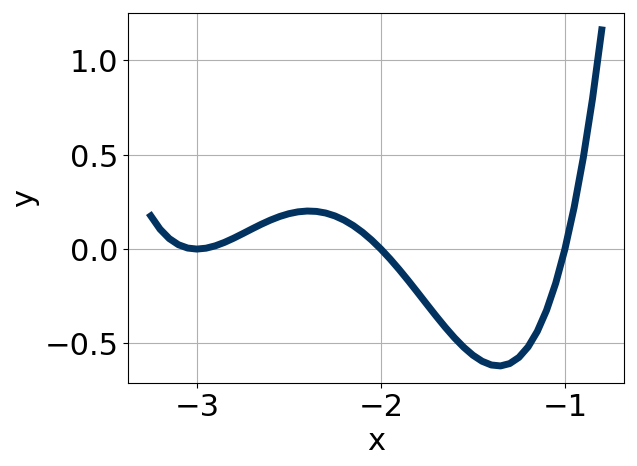
\includegraphics[scale=0.5]{../Figures/question26C.png}\end{center}The solution is $ (x + 3)^2(x + 2)(x + 1) $ 

\begin{enumerate}[label=\Alph*.] 
\item $ (x + 3)^2(x + 2)^2(x + 1) $ 

  
\item $ (x + 3)^2(x + 2)(x + 1) $ 

  
\item $ -(x + 3)^2(x + 2)(x + 1)^2 $ 

  
\item $ -(x + 3)^2(x + 2)(x + 1) $ 

  
\item $ (x + 3)(x + 2)^2(x + 1) $ 

  
\end{enumerate} 
 
General Comments: Draw the x-axis to determine which zeros are touching (and so have even multiplicity) or cross (and have odd multiplicity)

-----------------------------------------------

27. Choose the end behavior of the polynomial below.
$$ f(x) = 4(x + 2)^{3}(x - 2)^{6}(x - 6)^{2}(x + 6)^{2} $$ 
The solution is  
\begin{center}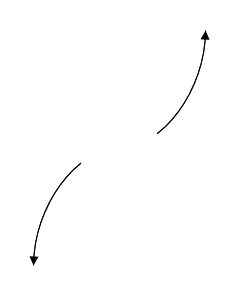
\includegraphics[scale=0.5]{../Figures/endBehaviorPositiveOdd.png}\end{center}\begin{enumerate}[label=\Alph*.] 
\item Negative leading coefficient, sum of degrees is odd. 
\begin{center}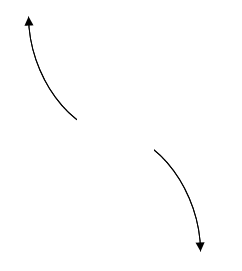
\includegraphics[scale=0.5]{../Figures/endBehaviorNegativeOdd.png}\end{center} 
 
\item Negative leading coefficient, sum of degrees is even. 
\begin{center}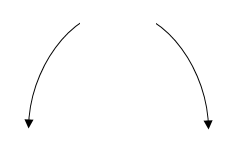
\includegraphics[scale=0.5]{../Figures/endBehaviorNegativeEven.png}\end{center} 
 
\item Positive leading coefficient, sum of degrees is even. 
\begin{center}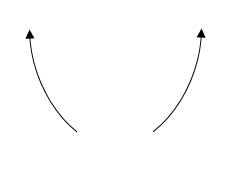
\includegraphics[scale=0.5]{../Figures/endBehaviorPositiveEven.png}\end{center} 
 
\item Positive leading coefficient, sum of degrees is odd. 
\begin{center}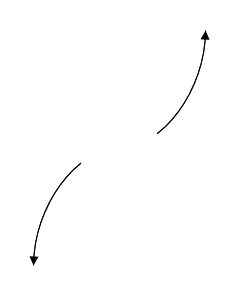
\includegraphics[scale=0.5]{../Figures/endBehaviorPositiveOdd.png}\end{center} 
 
\end{enumerate} 
 
General Comments: Remember that end behavior is determined by the leading coefficient AND the sum of the multiplicities.

-----------------------------------------------

28. Describe the zero behavior of the zero $x = -2$ of the polynomial below.
$$ f(x) = 4(x + 2)^{3}(x - 2)^{6}(x - 6)^{2}(x + 6)^{2} $$ 
The solution is  
\begin{center}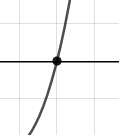
\includegraphics[scale=0.5]{../Figures/zeroBehaviorPositiveOdd.png}\end{center}\begin{enumerate}[label=\Alph*.] 
\item The function is above the $x$-axis, then passes through. 
\begin{center}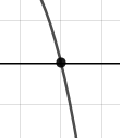
\includegraphics[scale=0.5]{../Figures/zeroBehaviorNegativeOdd.png}\end{center} 
 
\item The function is below the $x$-axis, then touches. 
\begin{center}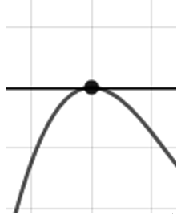
\includegraphics[scale=0.5]{../Figures/zeroBehaviorNegativeEven.png}\end{center} 
 
\item The function is above the $x$-axis, then touches. 
\begin{center}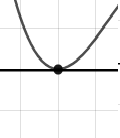
\includegraphics[scale=0.5]{../Figures/zeroBehaviorPositiveEven.png}\end{center} 
 
\item The function is below the $x$-axis, then passes through. 
\begin{center}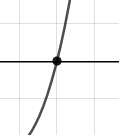
\includegraphics[scale=0.5]{../Figures/zeroBehaviorPositiveOdd.png}\end{center} 
 
\end{enumerate} 
 
General Comments: You will need to sketch the entire graph, then zoom in on the zero the question asks about.

-----------------------------------------------

29. Construct the lowest-degree polynomial given the zeros below. Then, choose the intervals that contain the coefficients of the polynomial in the form $ax^3+bx^2+cx+d$.
$$ \frac{7}{3}, -5, \text{ and } -2 $$ 
The solution is $ 3 x^3 + 14 x^2 - 19 x - 70 $ 

\begin{enumerate}[label=\Alph*.] 
\item $ a \in [0, 4], b \in [25, 30], c \in [77, 87], \text{ and } d \in [68, 71] $ 

  Distractor 3: This corresponds to using $(x+z_1)$ for the first term. 
\item $ a \in [0, 4], b \in [-6, 2], c \in [-52, -45], \text{ and } d \in [-71, -67] $ 

  Distractor 4: This corresponds to using $(x+z_1)(x+z_2)$ for the first two terms. 
\item $ a \in [0, 4], b \in [8, 20], c \in [-22, -16], \text{ and } d \in [-71, -67] $ 

 * This is the correct solution 
\item $ a \in [0, 4], b \in [8, 20], c \in [-22, -16], \text{ and } d \in [68, 71] $ 

  Distractor 2: This corresponds to having everything correct except the sign of the last term. 
\item $ a \in [0, 4], b \in [-17, -13], c \in [-22, -16], \text{ and } d \in [68, 71] $ 

  Distractor 1: This corresponds to multiplying $(x+z_1)(x+z_2)(x+z_3)$ 
\end{enumerate} 
 
General Comments: To construct the lowest-degree polynomial, you want to multiply out $(3x-7)(1x--5)(1x--2)$

-----------------------------------------------

30. Construct the lowest-degree polynomial given the zeros below. Then, choose the intervals that contain the coefficients of the polynomial in the form $x^3+bx^2+cx+d$.
$$ 4i \text{ and } -3 $$ 
The solution is $ x^3 + 3 x^2 + 16 x + 48 $ 

\begin{enumerate}[label=\Alph*.] 
\item $ b \in [-3.9, -2.2], c \in [-19, -12], \text{ and } d \in [-49, -41] $ 

  Distractor 4: This distractor corresponds to negatives for each of the coefficients in the solution. 
\item $ b \in [0.5, 2.2], c \in [1, 7], \text{ and } d \in [-3, 1] $ 

  Distractor 2: This distractor corresponds to using a from the complex and the other zero to make a quadratic. 
\item $ b \in [2.6, 5.2], c \in [11, 18], \text{ and } d \in [44, 53] $ 

 * This is the correct solution 
\item $ b \in [0.5, 2.2], c \in [-2, 0], \text{ and } d \in [-13, -8] $ 

  Distractor 3: This distractor corresponds to using b from the complex and the other zero to make a quadratic. 
\item $ b \in [-3.9, -2.2], c \in [11, 18], \text{ and } d \in [-49, -41] $ 

  Distractor 1: This distractor corresponds to using (x+z) for zeros. 
\end{enumerate} 
 
General Comments: Remember that the conjugate of $a+bi$ is $a-bi$. Since these zeros always come in pairs, we need to multiply out $(x-4i)(x+4i)(x--3)$

-----------------------------------------------


\end{document}
